\section{Application}
\label{sec:application}
%TMACS is still in early development phase and it has the functionality needed to perform modeling, formal specification, and verification of concurrent systems. 
In this chapter we demonstrate that process of formal specification and verification for 
%two classical problems in the concurrency theory: the alternating bit protocol and the mutual exclusion algorithm of Peterson.
one classical problem in the concurrency theory: the alternating bit protocol. The alternating bit protocol is a simple yet effective protocol (usually used as a test case), designed to ensure reliable communication through unreliable transmission mediums, and it is used for managing the retransmission of lost messages \cite{ReactiveSystems}\cite{Kulick}.

\subsection{Alternating bit protocol - modelling, specification and verification}

The alternating bit protocol is a simple yet effective protocol (usually used as a test case), designed to ensure reliable communication through unreliable transmission mediums, and it is used for managing the retransmission of lost messages \cite{ReactiveSystems}\cite{Kulick}.

\subsubsection{Modelling and Specification.}
The representation of the Alternating Bit Protocol consists of a $sender$ $S$, a $receiver$ $R$ and two channels $transport$ $T$ and $acknowledge$ $A$ as shown below. 

\begin{figure}[h]
\centering
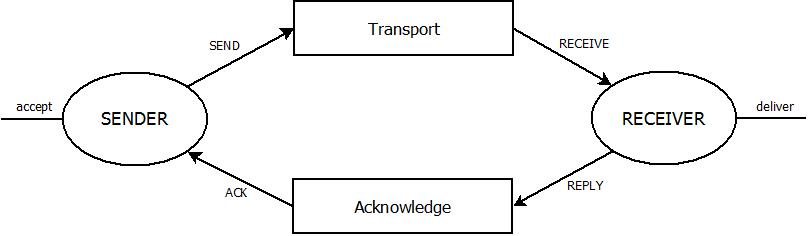
\includegraphics[width=4.5in]{abp}
\caption{Alternating Bit Protocol representation}
\label{fig:abp}
\end{figure}

The only visible transitions in the alternating bit protocol are $deliver$ and $accept$, which can occur only sequentially, whereas all others are internal synchronizations. Sender $S$ sends a message which contains the protocol bit, 0 or 1, to a receiver $R$. The channel from $S$ to $R$ is initialized and there are no messages in transit. There is no direct communication between the sender $S$ and the receiver $R$, and all messages must travel trough the medium ($transport$ and $acknowledge$ channel). 

The functioning of the alternating bit protocol can be described as follows \cite{ReactiveSystems}:
\begin{enumerate}
	\item The sender $S$ sends a message repeatedly (with its corresponding bit) until it receives an acknowledgment ($ack0$ or $ack1$) from the receiver $R$ that contains the same protocol bit as the message being sent. This behaviour of the process representing the sender can be described as:
				\begin{equation*}\label{send_imp}
				    \begin{array}{lcl}
							S = \overline{send0}.S+ack0.accept.S_{1}+ack1.S \\
							S_{1}=\overline{send1}.S_{1}+ack1.accept.S+ack0.S_{1}				  
						\end{array}
				\end{equation*}
	      The transport channel transmits the message to the receiver, but it may lose the message (lossy channel) or transmit it several times (chatty channel). Therefore, the description of the behaviour of the process representing the transport channel is given with CCS expression as follows:
	      \begin{equation*}\label{trans_imp}
	      	\begin{array}{lcl}
						T=send0.\left(T+T_{1}\right)+send1.\left(T+T_{2}\right)\\
						T_{1}=\overline{receive0}.\left(T+T_{1}\right)\\
						T_{2}=\overline{receive1}.\left(T+T_{2}\right)
					\end{array}
				\end{equation*}
  \item When the receiver $R$ receives a message, it sends a reply to $S$ which includes the protocol bit of the message received. When the message is received for the first time, the receiver will deliver it for processing, while subsequent messages with the same bit will be simply acknowledged. That yields the following CCS expression for the receiver:
  			\begin{equation*}\label{rec_imp}
				    \begin{array}{lcl}
							R=receive0.\overline{deliver}.R_{1}+\overline{reply1}.R+receive1.R \\
							R_{1}=receive1.\overline{deliver}.R+\overline{reply0}.R_{1}+receive0.R_{1}			  
						\end{array}
				\end{equation*}
        Again, the acknowledgement channel sends the $ack$ to sender, and it can also acknowledge it several times or lose it on the way to the sender. Therefore the CCS expression describing the ackowledgement channel and its behaviour is given as follows:
        \begin{equation*}\label{trans_imp}
	      	\begin{array}{lcl}
						A=reply0.\left(A+A_{1}\right)+reply1.\left(A+A_{2}\right)\\
						A_{1}=\overline{ack0}.\left(A+A_{1}\right)\\
						A_{2}=\overline{ack1}.\left(A+A_{2}\right)
					\end{array}
				\end{equation*}
  \item When $S$ receives an acknowledgment containing the same bit as the message it is currently transmitting, it stops transmitting that message, flips the protocol bit, and repeats the protocol for the next message.\cite{Kulick}\cite{ProcessAlgebraParallel}
\end{enumerate}

Having described the behaviour of the alternating bit protocol components, the CCS process expression describing the behaviour of the protocol as a whole can be obtained as a parallel composition of the processes describing the sender, the transport channel, the receiver and the acknowledgement channel:
\begin{equation}\label{abp_imp}
	\mathit{ABP} \stackrel{def}{=}\left(S|T|R|A\right)\backslash L,
\end{equation}
restricted on the set of actions:
\begin{equation*}
  L = \left(send0,send1,receive0,receive1,reply0,reply1,ack0,ack1\right)
\end{equation*}

This CCS expression represents the implementation of the alternating bit protocol which details the proposed means for achieving the desired high-level behaviour the alternating bit protocol should exhibit. This desired high-level behaviour is that the alternating bit protocol should act as a simple buffer, therefore its CCS specification is defined as follows:
\begin{equation}\label{eq:abp_spec}
	\begin{array}{lcl}
		\mathit{Buf} = \mathit{accept.Buf'}\\
		\mathit{Buf'} = \mathit{\overline{deliver}.Buf}
	\end{array}
\end{equation}

\subsubsection{Verification.} In order to verify the alternating bit protocol, we need to prove that the implementation $ABP$ meets the specification $Buf$ with respect to some behavioural equivalence. We shall show that an observational equivalence between $\mathit{Buf}$ and $\mathit{ABP}$ can be found, i.e. that $\mathit{ABP}\approx \mathit{Imp}$. For that purpose, first we use TMACS to obtain the labeled graphs corresponding to the CCS representations of $\mathit{Buf}$ and $\mathit{ABP}$, and afterwards we perform a comparison of the labeled transition systems modulo weak bisimilarity which yields a positive answer about the existance of weak bisimulation equivalence between $\mathit{Buf}$ and $\mathit{ABP}$.

The weak bisimulation equivalence obtained by running any of the two bisimulation algorithms implemented in TMACS over the saturated labeled transition systems is given in Table~\ref{table3}:

\begin{table}
\begin{tabular}{| p{6.5cm} | p{3.5cm} | }
	
  \hline                       
	ABP implementation states &
	ABP specification states
	\\ \hline
	
$\left(S|T|R|A\right)\backslash L$ & \\
$\left(S|\left(T+T1\right)|R|A\right)\backslash L$ & \\
$\left(S|\left(T+T1\right)|R|\left(A+A2\right)\right)\backslash L$ & \\
$\left(S|T|R|\left(A+A2\right)\right)\backslash L$ & \\
$\left(S|\left(T+T1\right)|\overline{deliver}.R1|A\right)\backslash L$ & \\
$\left(S|\left(T+T1\right)|\overline{deliver}.R1|\left(A+A2\right)\right)\backslash L$ & \\
$\left(S1|\left(T+T1\right)|R1|\left(A+A1\right)\right)\backslash L$ & \\
$\left(S1|\left(T+T2\right)|\overline{deliver}.R|\left(A+A1\right)\right)\backslash L$ & \\
$\left(S1|\left(T+T2\right)|R1|\left(A+A1\right)\right)\backslash L$ & \\
$\left(S|\left(T+T2\right)|R|\left(A+A2\right)\right)\backslash L$ &
  $\mathit{Buf}$   
  \\ \hline
   
$\left(accept.S1|\left(T+T1\right)|R1|\left(A+A1\right)\right)\backslash L$ & \\ 
$\left(S|\left(T+T1\right)|R1|\left(A+A1\right)\right)\backslash L$ & \\
$\left(S|\left(T+T1\right)|R1|\left(A+A2\right)\right)\backslash L$ & \\
$\left(S|\left(T+T1\right)|R1|A\right)\backslash L$ & \\
$\left(S1|\left(T+T2\right)|R|\left(A+A2\right)\right)\backslash L$ & \\
$\left(accept.S|\left(T+T2\right)|R|\left(A+A2\right)\right)\backslash L$ & \\
$\left(S1|\left(T+T2\right)|R|\left(A+A1\right)\right)\backslash L$ &
  $\mathit{Buf'}$
  \\ \hline  
\end{tabular}
\\
\caption{Verification of the alternating bit protocol using weak bisimilarity}
\label{table3}
\end{table}

%\subsection{Peterson's algorithm - modeling, specification and testing}

Peterson's algorithm \cite{Peterson} is a simple algorithm designed to ensure mutual exclusion (often abbreviated as mutex) between two processes without any special hardware support. It represents a simple refinement of ideas from earlier mutex algorithms such as Dekker's algorithm \cite{Dekker}. Mutual exclusion algorithms are used in concurrent programming to avoid the simultaneous use of a common resource by critical sections. A critical section is a piece of code in which a process or thread accesses a shared resource. 

\subsubsection{Modeling and Specification.}In Peterson's algorithm for mutual exclusion, there are \cite{ReactiveSystems}:
\begin{itemize}
  \item Two processes $P_{1}$ and $P_{2}$ that want to access the same resource, i.e. enter the critical section;
	\item Two shared variables $b_{1}$ and $b_{2}$ which indicate whether process $P_{1}$ and process $P_{2}$ are trying to enter the critical section;
	\item A shared integer variable $k$ that can take one of the values 1 or 2 and indicates which process is next to enter the critical section;
\end{itemize}

The boolean variables $b_{1}$ and $b_{2}$ are initialized to values $false$ because neither of the processes is interested yet to enter the critical section, whereas the initial value of $k$ is arbitrary. 

In order to ensure mutual exclusion, each process $P_{i}$, $i\in\left\{1,2\right\}$, executes the following algorithm presented in pseudocode, where $j$ denotes the index of the other process. 

\begin{algorithm}
\caption{Peterson's algorithm pseudocode}
\begin{algorithmic}
\WHILE{$true$} 
	\STATE $\left\langle noncritical \hspace{1mm} section \right\rangle$;  
	\STATE $b_{i} \gets true$;
	\STATE $k \gets j$;
	\WHILE {$\left(b_{j} \hspace{1mm} and \hspace{1mm} k = j\right)$}
		 \STATE skip;
	\ENDWHILE
	\STATE $\left\langle \mathit{critical} \mathit{section} \right\rangle$;
	\STATE $b_{i} \gets false$;
\ENDWHILE
\end{algorithmic}
\end{algorithm}

Modeling the algorithm of Peterson includes, among other tasks, translation of the pseudocode description of the behaviour of the processes $P_{1}$ and $P_{2}$ into CCS expressions or labeled transition systems. 

Following the message-passing paradigm on which CCS is based, the variables manipulated by the processes $P_{1}$ and $P_{2}$ are viewed as passive agents that react to actions performed by the processes. Therefore, the description of the variables used in Peterson's algorithm as processes can be done as follows \cite{ReactiveSystems}:
\begin{enumerate}
	\item The process representing the shared boolean variable $b_{1}$ has two states and its behaviour can be represented by the following CCS expressions:\\
				\begin{equation*}\label{b1_imp}
				    \begin{array}{lcl}
							B1f = \overline{b1rf}.B1f + b1wf.B1f + b1wt.B1t \\
							B1t = \overline{b1rt}.B1t + b1wf.B1f + b1wt.B1t			  
						\end{array}
				\end{equation*}
	      Similarly for the process describing the behaviour of the variable $b_{2}$:\\
	      \begin{equation*}\label{b2_imp}
				    \begin{array}{lcl}
							B2f = \overline{b2rf}.B2f + b2wf.B2f + b2wt.B2t \\
							B2t = \overline{b2rt}.B2t + b2wf.B2f + b2wt.B2t,		  
						\end{array}
				\end{equation*}
	      where the pattern for the channel name is $b<i><x><y>$, with:
	      \begin{itemize}
					\item $i\in\left\{1,2\right\}$ for the process ID
					\item $x\in\left\{r,w\right\}$ for the type of operation (read or write)
					\item $y\in\left\{f,t\right\}$ for the variable value to be written or read (false or true)
				\end{itemize}
	\item The process representing the variable $k$ has two states, denoted by the constants $K_{1}$ and $K_{2}$, because the variable $k$ can only take one of the two values 1 and 2, and its CCS representation is as follows\\
				\begin{equation*}\label{k_imp}
				    \begin{array}{lcl}
							K1 = \overline{kr1}.K1 + kw1.K1 + kw2.K2 \\
							K2 = \overline{kr2}.K2 + kw2.K2 + kw2.K2,		  
						\end{array}
				\end{equation*}
				where the pattern for the channel name is $k<x><n>$, with:
			  \begin{itemize}
					\item $x\in\left\{r,w\right\}$ for the type of operation (read or write)
					\item $n\in\left\{1,2\right\}$ for the value to be written or read
				\end{itemize}
\end{enumerate}

The final step is the CCS formalisation of the behaviour of the processes $P_{1}$ and $P_{2}$. The process behaviour outside of the critical region can be ignored and the focus can be put on the process entering and exiting the critical section. Under the assumption that the processes cannot fail or terminate within the critical section, the initial behaviour of the process $P_{1}$ can be described by the following CCS expression:\\
				\begin{equation*}\label{p1_imp}
				    P1 = \overline{b1wt}.\overline{kw2}.P11,
				\end{equation*}
				where $P11$ models the while loop (with short-circuit evaluation):
				\begin{equation*}\label{p11_imp}
				    P11 = b2rf.P12 + b2rt.\left(kr2.P11 + kr1.P12\right)
				\end{equation*}
				and $P12$ models the critical section:
				\begin{equation*}\label{p12_imp}
				    P12 = enter1.exit1.\overline{b1wf}.P1
				\end{equation*}

The behaviour of the process $P_{2}$ can be described with CCS expressions in the similar manner:
				\begin{equation*}\label{p2_imp}
				    \begin{array}{lcl}
							P2 = \overline{b2wt}.\overline{kw1}.P21 \\
							P21 = b1rf.P22 + b1rt.\left(kr1.P21 + kr2.P22\right)\\
							P22 = enter2.exit2.\overline{b2wf}.P2	  
						\end{array}
				\end{equation*}

The CCS process expression representing Peterson's algorithm as a whole consists of the parallel composition of the terms describing the two processing running the algorithm and of those describing the variables. Since we are only interested in the behaviour of the algorithm pertaining to the access to, and exit from, their critical sections, all the communication channels that are used to read from, and write to the variables, are restricted:
\begin{equation*}
	L = \left\{b1rf,b1rt,b1wf,b1wt,b2rf,b2rt,b2wf,b2wt,kr1,kw1,kr2,kw2\right\}
\end{equation*}

Assuming that the initial value of the variable $k$ is 1, the implementation of Peterson�s algorithm is therefore given by the term:
\begin{equation}\label{pet_imp_full}
	PETERSON \stackrel{def}{=} \left(B1f|B2f|K1|P1|P2\right)\backslash L
\end{equation}

This process term details the proposed means for achieving the desired high-level behavior of Peterson's algorithm which is as of any simple mutex algorithm. Initially, both processes enter their critical sections, however once one of the processes has entered its critical section, the other process cannot enter its own critical section until the first process has exited its critical section. Therefore, a suitable CCS specification of the behaviour of a mutual exclusion algorithm like Peterson's is given as follows:
\begin{equation}
	MutexSpec = enter1.exit1.MutexSpec + enter2.exit2.MutexSpec
\end{equation}

\subsubsection{Testing.} One of the approaches that can be used to establish the correctness of the Peterson's algorithm is by testing the preservation of the mutual exclusion property. A test is a finite rooted labeled transition system over the set of actions $Act\cup\left\{\overline{bad}\right\}$, where $bad$ is a distinguished channel name not occurring in $Act$. The idea is that the test would act as a monitor process that 'observes' the behaviour of the processes and reports an error in case an undesirable situation occurs by performing a $bad$-labelled transition. Assuming that the monitor process outputs 'bad' when it discovers that two enter actions have occurred without intervening exit, a CCS process describing this behaviour is \cite{ReactiveSystems}:
\begin{equation*}\label{mut_test}
  \begin{array}{lcl}
  	MutexTest = \overline{enter1}.MutexTest1 + \overline{enter2}.MutexTest2 \\
		MutexTest1 = \overline{exit1}.MutexTest + \overline{enter2}.\overline{bad}.0\\
		MutexTest2 = \overline{exit2}.MutexTest + \overline{exit1}.\overline{bad}.0
	\end{array}
\end{equation*}

In order to check whether process $PETERSON$ ensures mutual exclusion, it is now sufficient to let it interact with $MutexTest$ and use TMACS to see if the resulting system
\begin{equation}\label{pet_test}
	\left(PETERSON|MutexTest\right)\backslash M,
\end{equation}
where 
\begin{equation*}
	M = \left\{enter1,enter2,exit1,exit2\right\},
\end{equation*}
can initially perform the action $\overline{bad}$.

Indeed, the labeled transition system of the above CCS expression generated by TMACS does not have states which afford $bad$ transitions. This proves that Peterson's algorithm ensures mutual exclusion.